
\myChapter{Access Control e Usage Control}
\label{cap:accessControl}
I sistemi informatici moderni sono capaci di condividere dati e
risorse computazionali, ed impedire accessi non autorizzati è diventata
una priorità inderogabile.
I motivi che portano a questa decisione possono essere legati alla privacy o alla consistenza dei dati durante una computazione.
Ad esempio, molte informazioni personali possono essere
raccolte durante alcune attività quotidiane, dunque diventa necessario
proteggere questi dati da malintenzionati. Per questo motivo esistono sistemi di Access Control, ovvero dei sistemi
definiti da un insieme di condizioni che permettono di creare una prima
linea difensiva contro accessi indesiderati.


Nella prima parte di questo capitolo vengono trattati in maggior dettaglio i vari modelli 
di controllo all'accesso proposti negli ultimi decenni, infine viene analizzato anche un nuovo modello chiamato \textit{Usage Control}.

\section{Access Control}
\label{sec:history}



Negli anni sono stati proposti diversi approcci per cercare di definire un
modello efficiente e scalabile. Andremo ora ad eseguire una classificazione
dei modelli di Access Control, seguendo la catalogazione del NIST \cite{NISTACM}.

\begin{itemize}
\item \acl{ACL} è il primo di questi modelli ed è stato proposto intorno al 1970 spinto
dall’avvento dei primi sistemi multi utente.
\item \acl{RBAC} è nato successivamente ad \ac{ACL} e ne modifica alcuni aspetti in modo da rimuovere
molte delle limitazioni di quest’ultimo. 
\item \acl{ABAC} è nato dopo \ac{RBAC} e fornisce un paradigma dinamico che aiuta a 
\item \acl{PBAC} è molto simile ad \ac{ABAC} ma migliora e standardizza quest ultimo modello.

\end{itemize}

\subsection*{Access Control Lists (ACLs)}
\label{sub:ACL}

\ac{ACL} è il primo modello di controlli agli accessi, è stato introdotto intorno agli anni 70 grazie all'avvento dei sistemi multi utente allo scopo di limitare l'accesso a file e dati condivisi, infatti i primi sistemi ad utilizzare questo modello sono stati sistemi di tipo UNIX. Con la comparsa della multiutenza per sistemi ad uso personale lo standard ACL è stato implementato in molte più ambienti come sistemi UNIX-Like e Windows. \par
Il concetto dietro ACL è uno dei più semplici, in quanto ogni risorsa del sistema che deve essere controllata ha una sua lista, che ad ogni soggetto associa le azioni che può effettuare sulla risorsa, ed il sistema operativo quando viene fatta richiesta decide in base alla lista se dare il permesso o meno. 


Per esempio in Figura \ref{fig:acl_osx}, si può vedere come \textit{test\_folder} sia la risorsa da controllare, \textit{federicoschipani}, \textit{staff} e \textit{everyone} siano i soggetti e le azioni associate sono, in questo caso, \textit{Read \& Write} al primo soggetto e \textit{Read only} agli altri due.
\MyFig{acl_osx}{ACL in OS X}{0.8}{h}


La semplicità di questo modello non richiede grandi infrastrutture sottostanti, la  sua implementazione dal punto di vista applicativo risulta abbastanza semplice attraverso l'uso di linguaggi ad alto livello come Python o Java, poiché le strutture che servono per implementare questo standard sono già definite.
Nonostante negli anni sono stati sviluppati modelli più complessi, come \ac{ABAC}, \ac{PBAC} e \ac{RBAC}, il sistema descritto in questa sezione viene comunque usato nei sistemi operativi recenti. Come si può vedere in Figura \ref{fig:acl_osx} OS X sfrutta questo standard per la gestione dei permessi sul filesystem. \par
Un aspetto negativo si manifesta quando si trattano grandi quantità di risorse. Ogni volta che viene richiesto l'accesso ad una risorsa da parte di un entità, utente o applicazione che sia, è necessario verificare nella lista associata, il che lo rende abbastanza oneroso dal punto di vista computazionale. \par
Un altro lato negativo emerge quando bisogna effettuare modifiche ai permessi di una determinata risorsa, in quanto è necessario andare ad operare sulla lista di quest'ultima, il che rende questo compito incline ad errori ed oneroso dal punto di vista del tempo.


\subsection*{Role-based Access Control (RBAC)} % (fold)
\label{sub:role_based_access_control}

RBAC è l'evoluzione di ACL, in quanto tende a correggerne alcuni difetti come la limitata scalabilità. \par
A differenza di \ac{ACL} è presente il concetto il ruolo del richiedente, ovvero un titolo che definisce un livello di autorità, che raggrupperà diversi utenti in una categoria. 
\ac{RBAC} attraverso questa nuova caratteristica riesce a porre rimedio ai difetti di \ac{ACL} in quanto
questo tipo di gestione offre il vantaggio di facilitare l'assegnazione dei permessi, poiché per ogni risorsa non si devono più gestire tutti i singoli utenti, ma basta gestire i permessi associati a queste nuove categorie. 


Un utente può anche far parte di più gruppi, per esempio un contabile di un azienda può far parte del gruppo \textit{impiegati} e \textit{contabili} in modo da permettergli l'accesso sia ai documenti riservati ai soli impiegati che quelli riservati ai soli contabili.
Come si può vedere in Figura \ref{fig:group2} il concetto di gruppo è implementato nei sistemi operativi moderni, in particolare in OS X, Windows e sistemi UNIX-Like.

\MyFig{group2}{Gruppo in OS X}{0.9}{h}
\ac{RBAC} però ha i suoi difetti, uno dei più evidenti è l'impossibilità di gestire le autorizzazioni a livello di singola persona, ed è quindi necessario creare diversi gruppi o trovare altri escamotage\footnote{Gioco di destrezza con cui si sottrae qualche cosa all’attenzione degli interessati o dei presenti, gioco di bussolotti; in senso fig., inganno elegante o ingegnoso, gioco di abilità politica e diplomatica, o in genere sotterfugio per aggirare un ostacolo} per autorizzare, o vietare, singoli utenti appartenti a determinati gruppi.

% subsection role_based_access_control (end)

\subsection*{Attribute-based Access Control (ABAC)} % (fold)
\label{sub:attribute_based_access_control_}

\ac{ABAC} è un modello di controllo all'accesso  nel quale le decisioni sono prese in base ad un insieme 
di attributi, associazioni con il richiedente, ambiente e risorsa stessa.
In questa nuova architettura è presente un nuovo componente chiamato \ac{PDP} il quale si occuperà della valutazione delle richieste prima di fornire una decisione finale.
Ogni attributo è un campo distinto dagli altri che il \ac{PDP} compara con un insieme di valori per determinare o meno l'accesso alla risorsa. 

In Figura~\ref{fig:ABAC} viene mostrato il funzionamento di \ac{ABAC}. Di particolare rilevanza è il secondo step, che porta alla raccolta di tutte le informazioni per produrre una decisione finale.
Inizialmente il sistema richiede al \ac{ACS} le policy, successivamente effettua la raccolta degli attributi dalle varie fonti.
\MyFig{ABAC}{Scenario ABAC base}{0.8}{} %SOSTITUIRE CON GRAFICO SIMILE
Questi attributi possono provenire da disparate fonti ed essere di svariati tipi. Per esempio nella valutazione di una richiesta possono essere considerati attributi come la data di assunzione di un dipendente ed il suo grado all'interno dell'azienda. 


Un vantaggio di \ac{ABAC} è che non c'è la necessità che il richiedente conosca in anticipo
la risorsa o il sistema a cui dovrà accedere. Fino a quando gli attributi che il richiedente fornisce 
coincidono con i requisiti dettati dalle policy l'accesso sarà garantito. \ac{ABAC} perciò è utilizzato in situazioni in 
cui i proprietari delle risorse vogliono far accedere utenti che non conoscono direttamente a patto che però rispettino i criteri preposti, il che rende il tutto molto più dinamico rispetto ad \ac{ACL} e \ac{RBAC} \par
Diversamente da \ac{ACL} e \ac{RBAC} questo tipo di controllo agli 
accessi non è implementato nei sistemi operativi, ma è largamente usato a livello applicativo.
Spesso si usano applicazioni intermedie per mediare gli accessi da parte degli utenti a specifiche risorse.
Implementazioni semplici di questo modello non richiedono grandi \textit{database} o altre infrastrutture, tuttavia in ambienti dove non basta una semplice applicazione c'è necessità di grandi banche di dati.\par
Una limitazione di \ac{ABAC} è che in grandi ambienti, con tante risorse, individui e applicazioni ci saranno molte regole, ed organizzarle in maniera efficiente diventa un compito oneroso.


\subsection*{Policy-based Access Control (PBAC)} % (fold)
\label{sub:policy_based_access_control_}

\ac{PBAC} è stato sviluppato per far fronte alle problematiche di organizzazione delle regole di \ac{ABAC}, infatti è una sua naturale evoluzione e tende ad uniformare ed armonizzare il sistema di controllo accessi.
Questo modello cerca di aiutare le imprese a indirizzarsi verso la necessità di implementare un sistema di controllo agli accessi basato su policy.\par
\ac{PBAC} combina attributi dalle risorse, dall'ambiente e dal richiedente con informazioni su determinate circostanze sotto le quali la richiesta è stata effettuata ed inoltre si serve di 
ruoli per determinare quando garantire l'accesso.\par
Nei sistemi \ac{ABAC} gli attributi richiesti per avere accesso ad una particolare risorsa sono determinati a livello locale e possono variare da organizzazione ad organizzazione.
Per esempio, un'unità organizzativa può determinare che l'accesso ad un archivio di documenti sensibili è semplicemente soggetto a richiesta di credenziali e ruolo particolare.
Un'altra unità invece, oltre a richiedere credenziali e ruolo, richiede anche un certificato. Se un documento viene trasferito dal secondo al primo archivio perde la protezione fornita da quest'ultimo e sarà soggetto solo alla richiesta di credenziali e ruolo.
Con \ac{PBAC} invece si ha un solo punto dove vengono gestite le policy, e queste policy verranno valutate ad ogni tentativo di accedere alla risorsa.\par
\ac{PBAC} quindi è un sistema molto più complicato di \ac{ABAC} e perciò richiede il dislocamento di infrastrutture molto più onerose dal punto di vista economico che includono \textit{database}, \textit{directory service} e altri applicativi di mediazione e gestione.
\ac{PBAC} non richiede solo un applicazione per gestire la valutazione delle policy, ma
anche un sistema per la scrittura di queste ultime in modo che
non risultino ambigue.
Uno standard basato su \ac{XML}, e che si chiama \ac{XACML}, è sviluppato in modo tale da creare policy facilmente leggibili da una macchina. \par

Sfortunatamente però, queste policy non sono facili da scrivere e l’uso
di \ac{XACML} non necessariamente rende facile il processo di creazione, specifica e valutazione corretta di una policy. \par
Ci vorrebbe anche un modo per assicurarsi che tutti gli utenti di un sistema utilizzino lo stesso insieme di attributi, piuttosto arduo da realizzare. Gli attributi dovrebbero essere forniti da un’entità chiamata
\ac{AAS} che, oltre a fare da sorgente per gli
attributi, deve anche occuparsi della loro consistenza. In più bisogna instaurare
un meccanismo per verificare che questi attributi provengano
realmente dall’\ac{AAS}. Può sembrare facile fare una cosa del genere, ma
bisogna considerare il caso in cui più aziende lavorano insieme e devono
implementare un sistema di controllo degli accessi in comune. Un problema
si può verificare quando un’azienda valuta la gestione dell’\ac{AAS}
tramite una particolare \textit{repository}, ma un’altra azienda non è d’accordo a
questo tipo di soluzione

\section{Usage Control} % (fold)
\label{sec:usage_control}
Oggi sono presenti differenti tipi di sistemi diversi che richiedono un modello più flessibile e continuativo per gestire la sicurezza. Questa sezione parlerà di un nuovo sistema, chiamato \textit{Usage Control} \cite{SurveyUsageControl}. \par
\textit{Usage Control} si propone come un nuovo e promettente approccio per il controllo degli accessi. In particolare verrà trattato il modello, inizialmente proposto da Sandhu e Park\cite{SurveyUsageControl}, chiamato $UCON_{ABC}$. \par
$UCON_{ABC}$ utilizza un approccio diverso rispetto a \textit{Access Control} in quanto, rispetto a quest ultimo, si riesce ad avere una continuità delle decisioni sull'accesso. Ciò vuol dire che le decisioni non vengono più prese decisioni solo a priori, ma anche durante l'accesso.  Quindi, se durante l'utilizzo, qualche attributo di stato cambia e la \textit{policy} non è più soddisfatta viene revocato l'accesso. Di conseguenza è richiesto un componente che modella lo stato del sistema, in modo tale da effettuare valutazioni in base a quelle effettuate in precedenza. \par
Il vantaggio di \textit{Usage Control} è la sua capacità di adattarsi a vari casi di utilizzo, riuscendo così a includere e migliorare sistemi come \ac{ACL}, \ac{RBAC}, \ac{ABAC} e \ac{PBAC} descritti in \ref{sec:history}.
Il passaggio da Access Control a Usage Control è importante soprattutto quando si va a considerare ambienti legati alla rete, come possono essere il web o il cloud. \par
Il processo decisionale in Usage Control è diviso in due fasi \cite{UsageControlCloud}. 
\begin{itemize}
\item La prima fase è una fase di \textit{pre decision} che fondamentalmente è la classica decisione presa in \textit{Access Control}, questa decisione viene presa al momento in cui è effettuata la prima richiesta per produrre la decisione di accesso.
\item La seconda fase è chiamata \textit{ongoing decision}, ed è un processo che implementa il concetto di continuità in quanto le decisioni vengono prese durante l'accesso.\par
\end{itemize}
I componenti necessari a questo tipo di processo decisionale sono dei predicati, che possono essere di tre tipi, \textit{authorizations}, \textit{conditions} oppure \textit{rights}, delle azioni chiamate \textit{obligations} che devono essere eseguite durante l'accesso ed infine uno stato. 
\MyFig{Usage}{Insieme dei componenti di $UCON_{ABC}$}{1}{}
 Come questi componenti contribuiscono a prendere una decisione viene mostrato in Figura \ref{fig:Usage}.


\subsection{Caso di studio 1: Gestione lettura e scrittura di file} % (fold)

Dentro ad un sistema ci sono vari file, ai quali per questione di consistenza, bisogna limitare l'accesso.
La regola è: \textit{”per un determianto file un massimo di due persone possono accedere in lettura oppure solo una persona può accedere in scrittura"}. In Figura~\ref{fig:diagrammaflussoprimoesempio} viene mostrato un diagramma di flusso che sintetizza, e permette di capire meglio, la regola di accesso. Quando arriva la richiesta viene verificata la presenza nel database del richiedente e del file richiesto, se entrambe danno esito positivo si passa all'analisi dei requisiti per soddisfare la richiesta. \par
\begin{figure}[h]
 \centering 

 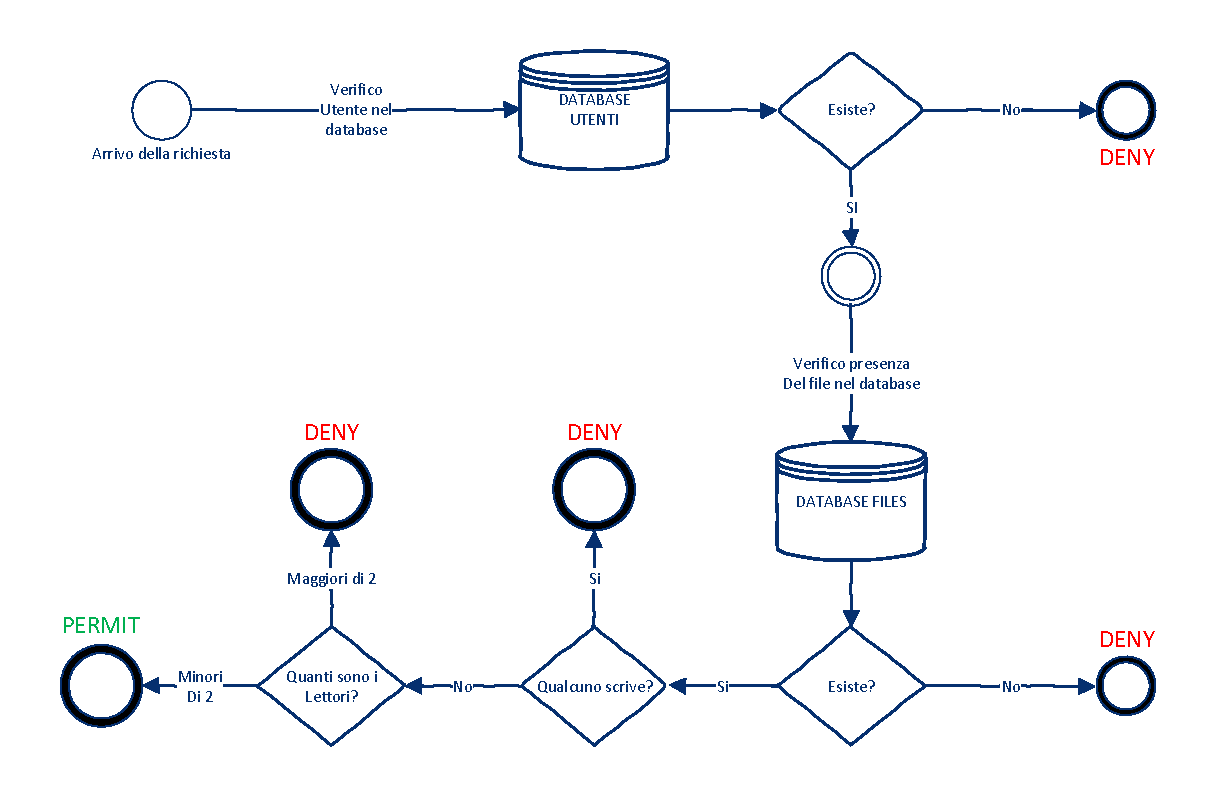
\includegraphics[scale = 0.75, , trim=1.5cm 0 0 0]{./Visio_Project/DiagrammaFlussoPrimoEsempio.pdf}
 \caption{Diagramma di flusso del primo esempio}
 \label{fig:diagrammaflussoprimoesempio}
\end{figure}
In un primo momento nessuno sta visualizzando o scrivendo un determinato file, ed un utente generico 
chiederà l'accesso in lettura per questo file, ovviamente il responso sarà positivo in quanto non viola la regola preposta prima.\par
Dopo un po' di tempo, mentre il primo sta ancora leggendo, un altro utente chiede l'accesso in scrittura, che gli viene negato.
In un istante di tempo successivo il primo utente sta continuando a leggere, ed anche il secondo utente vuole leggere. In questo caso viene dato responso positivo.\par
Infine, entrambi gli utenti smettono di leggere, ma uno di loro vuole apportare una modifica, allora richiede l'accesso in scrittura, che questa volta gli viene consentito poiché nessuno sta leggendo.



\subsection{Caso di studio 2: Noleggio e acquisto di contenuti}
Un altro utilizzo possibile di \textit{Usage Control} riguarda l'analisi del comportamento passato. Un'azienda fornisce  ai propri clienti 
la possibilità di effettuare noleggi o acquisti di contenuti multimediali (musica, video, film, serie tv e via discorrendo).\par
In caso il contenuto fosse stato acquistato, l’acquirente potrà ottenere
l’accesso infinite volte per infinito tempo. Nel caso di noleggio invece
saranno presenti delle condizioni, come per esempio il massimo numero
di fruizioni del contenuto o una data di scadenza che, una volta oltrepassata,
impedirà l’ulteriore visione del contenuto noleggiato in precedenza.\par
Come nell’esempio precedente viene proposto un diagramma di flusso,
proposto Figura~\ref{fig:diagrammaflussosecondoesempio}, che permette di capire meglio il funzionamento questo sistema di \textit{Usage Control}. Innanzitutto viene verificata la presenza nei due relativi database dell'utente e del file richiesto, successivamente viene analizzata la richiesta, che può essere di tre tipi.
\begin{itemize}
\item Visione: nel caso la richiesta fosse di visione viene verificato se realemente l'utente ha diritto ad avere accesso a quella risorsa, e di conseguenza viene presa una decisione.
\item Acquisto: nel caso la richiesta fosse di acquisto verrà accreditato l'acquisto all'utente che ha effettuato la richiesta.
\item Noleggio: per questa forma ci sono due diverse tipologie, il noleggio a tempo e il noleggio a numero di visualizzazioni. Nel primo caso all'utente sarà concesso di vedere il file per un determinato periodo di tempo, mentre nel secondo il richiedente potrà visionare il file per un numero limitato di volte.
\end{itemize}
\begin{figure}[h]
 \centering 
	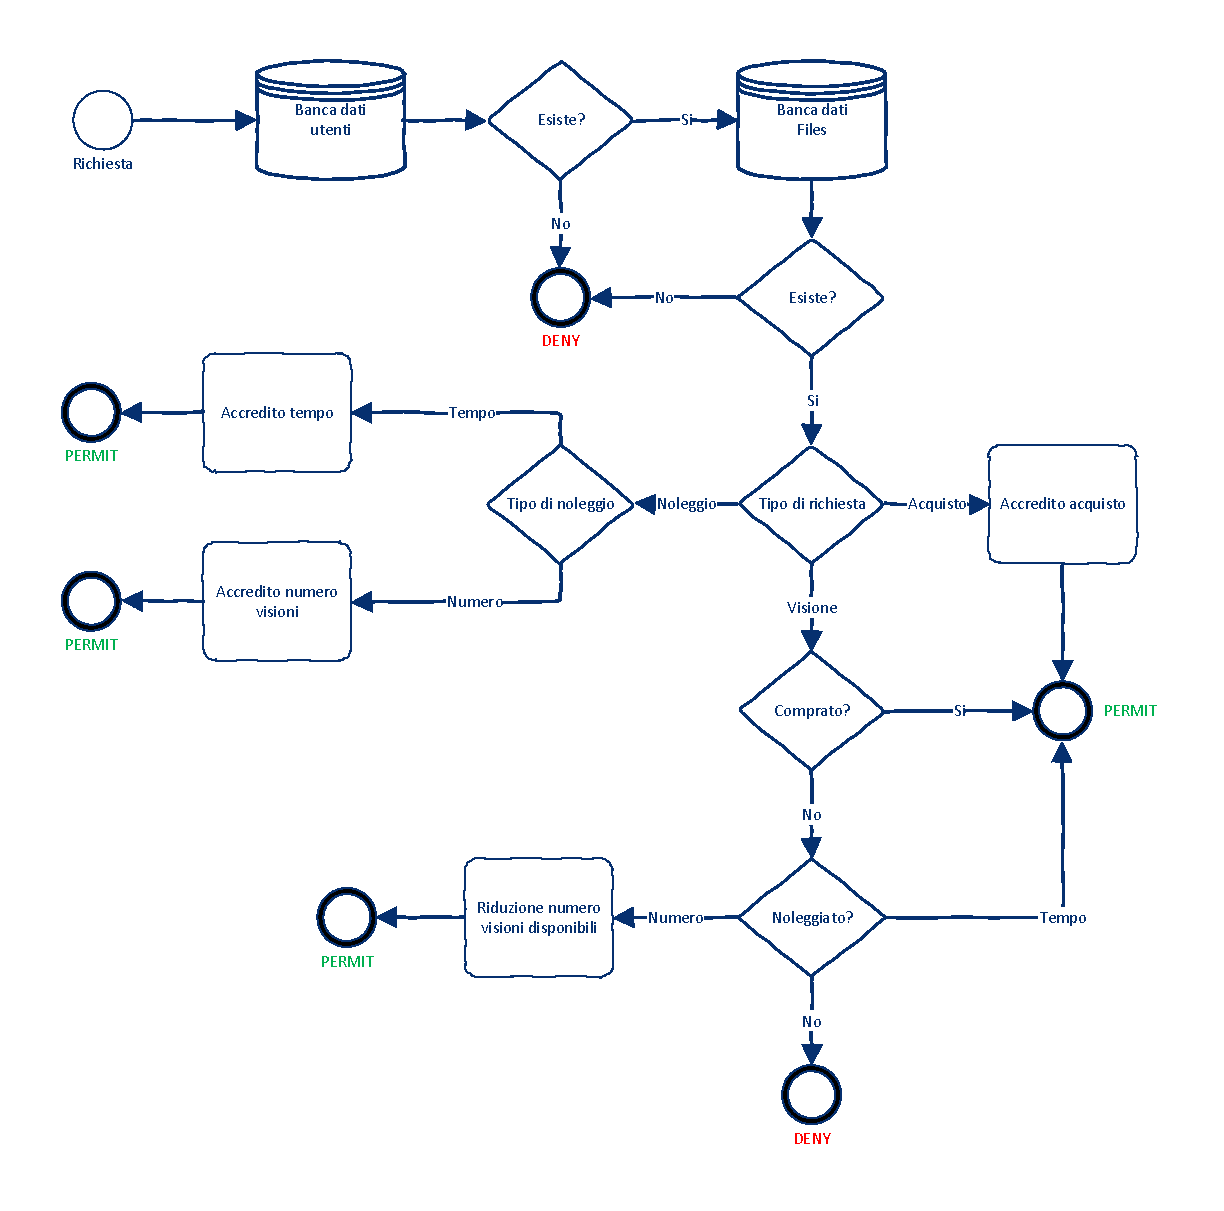
\includegraphics[scale = 0.75]{./Visio_Project/DiagrammaFlussoSecondoEsempio.pdf}
 \caption{Diagramma di flusso del secondo esempio}
 \label{fig:diagrammaflussosecondoesempio}
\end{figure}
